% Source: graduate-coursework/Sp26/CSCE763/Course_Assignments/HW2/HW2_CSCE_763_solutions.tex

\documentclass[border=4pt]{standalone}
\usepackage{amsmath}
\usepackage{amssymb}
\usepackage{graphicx}
\usepackage{tikz}
\usepackage{xcolor}
\usetikzlibrary{shapes.geometric, arrows.meta, positioning, patterns, calc}

\definecolor{USC_Garnet}{HTML}{73000A}
\definecolor{USC_Sandstorm}{HTML}{FFF2E3}
\definecolor{USC_Black90}{HTML}{363636}
\definecolor{USC_Black70}{HTML}{5C5C5C}
\definecolor{USC_Black50}{HTML}{A2A2A2}
\definecolor{USC_Black10}{HTML}{ECECEC}
\definecolor{USC_Honeycomb}{HTML}{65780B}
\definecolor{USC_Atlantic}{HTML}{466A9F}
\definecolor{USC_Congaree}{HTML}{1F414D}
\definecolor{USC_Rose}{HTML}{CC2E40}
\definecolor{USC_Grass}{HTML}{CED318}
\definecolor{USC_Horseshoe}{HTML}{65780B}
\definecolor{outputbg}{RGB}{245,245,245}

\begin{document}
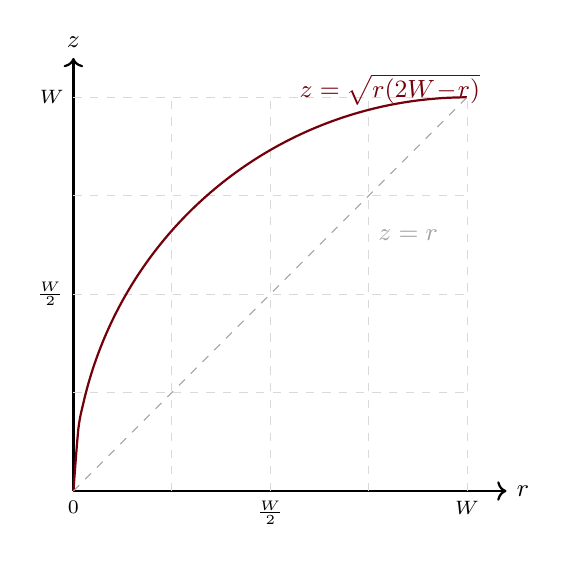
\begin{tikzpicture}[scale=5]
% Axes
\draw[->, thick] (0,0) -- (1.1,0) node[right, font=\small] {$r$};
\draw[->, thick] (0,0) -- (0,1.1) node[above, font=\small] {$z$};
% Grid
\foreach \v in {0.25,0.5,0.75,1.0} {
  \draw[dashed, gray!30] (\v,0) -- (\v,1);
  \draw[dashed, gray!30] (0,\v) -- (1,\v);
}
% Tick labels
\node[below, font=\scriptsize] at (0,0) {$0$};
\node[below, font=\scriptsize] at (0.5,0) {$\frac{W}{2}$};
\node[below, font=\scriptsize] at (1,0) {$W$};
\node[left, font=\scriptsize] at (0,0.5) {$\frac{W}{2}$};
\node[left, font=\scriptsize] at (0,1) {$W$};
% Quarter-circle arc: z = sqrt(r(2-r)), r in [0,1]
\draw[thick, USC_Garnet, domain=0:1, samples=80, smooth] plot (\x, {sqrt(\x*(2-\x))});
% Identity line
\draw[dashed, USC_Black50] (0,0) -- (1,1);
% Labels
\node[USC_Garnet, font=\small\bfseries, anchor=west] at (0.55,1.02) {$z = \sqrt{r(2W\!-\!r)}$};
\node[USC_Black50, font=\small, anchor=west] at (0.75,0.65) {$z = r$};
\end{tikzpicture}
\end{document}
